\documentclass[10pt,twocolumn]{article}

% use the oxycomps style file
\usepackage{oxycomps}

% usage: \fixme[comments describing issue]{text to be fixed}
% define \fixme as not doing anything special
\newcommand{\fixme}[2][]{#2}
% overwrite it so it shows up as red
\renewcommand{\fixme}[2][]{\textcolor{red}{#2}}
% overwrite it again so related text shows as footnotes
%\renewcommand{\fixme}[2][]{\textcolor{red}{#2\footnote{#1}}}

% read references.bib for the bibtex data
\bibliography{references}


% include metadata in the generated pdf file
\pdfinfo{
    /Title (Creating a Bunny Hop Trainer)
    /Author (Nico Cantrell)
}

% set the title and author information
\title{Bunny Hop Trainer Comps Proposal}
\author{Nico Cantrell}
\affiliation{Occidental College}
\email{ncantrell@oxy.edu}

\begin{document}

\maketitle
\section{Problem Context}
Video games as a hobby can be very difficult to approach. Tutorials provided in-game that are intended to teach new players how to play the game oftentimes assume that the player is familiar with the genre or commonly used techniques in similar games. The trainer in this paper focuses on teaching a mechanic in the video game Counter-Strike. In Counter-Strike, there are two numbers that appear at the bottom of the screen: one for health and one for ammo remaining in a weapon. While players familiar with the genre can understand what these numbers mean intuitively, this is not clear for new players. While it only takes a few minutes to understand how health works, there are many more complex systems in these games that can take hundreds of hours to master. 

One such complex mechanic present in Counter-Strike is a movement mechanic called bunny hopping. Bunny hopping is a technique where users perform a series of complicated aerial movements combined with a series of jumps that are triggered each time the user touches the ground. This technique makes the in-game character appear to jump similarly to a bunny and allows the user to gain and retain a significant amount of movement speed \cite{BunnyHoppingProgrammers}. This useful technique is not explicitly identified in the tutorial the game. Several online tutorials exist to teach players how to bunny hop, but these video tutorials often assume significant prior knowledge for the individual and do not give users concrete suggestions on how to improve specific to them \cite{QuakeBHopTutorial}. The technique of bunny hopping requires knowledge and execution of several advanced movement techniques at the same time. When I learned how to bunny hop, I had to use multiple different tutorials and ultimately try things out by myself. If I was not so dedicated to learning, it would have been very discouraging, and I want to make a tool I wish that I had access to. The goal of this project is to create a bunny hop trainer that teaches new users who are unfamiliar with the technique how to execute it with concrete feedback. Users are expected to use this tool for a short period, about twenty minutes each day for a week, in order to build familiarity with the technique.

\begin{figure}
    \centering
    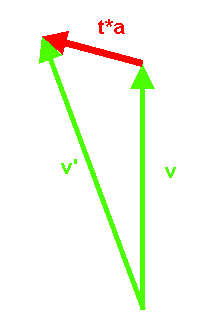
\includegraphics[width=0.5\linewidth]{figure2.png}
    \caption{Mouse movement for air strafing \cite{MoreSteamAirstrafe}}
\end{figure}

\section{Technical Background}


The main technical aspects of the bunny hop trainer revolve around emulating the physics engines present in Counter-Strike that make bunny hopping possible. The main mechanic that makes movement acceleration possible is a technique called air strafing. While bunny hopping in a straight line is useful to keep the momentum of a player, air strafing is the main way in which players gain that increased momentum. Air strafing is performed by moving the mouse left, causing the player character to look left while holding the left movement key or looking right while holding the right movement key \cite{AirStrafingExplained}. Counter-Strike's movement engine, the source engine, is heavily based on the Quake movement engine and air strafing is a consequence of an interesting decision on how velocity and acceleration is calculated \cite{AirStrafingExplained}. Limiting player speed is important for controlling how a game will play as it dictates where players will encounter one another and limits the scope of engagements. Many games limit player speed by directly limiting velocity, ensuring that players can never reach greater speeds than the designers intended. In the Quake and Counter-Strike acceleration systems, only the projection of the current velocity onto acceleration is limited \cite{BunnyHoppingProgrammers}.


When pressing the movement keys in source engine games, the engine used in Counter-Strike, the speed of the player is calculated each logical frame of the game. These logical frames are often called "ticks" and while a user can visually move locally in between ticks, their movement is only actually calculated every tick. Each logical frame, the game adds the acceleration vector in the direction the player's movement keys are being input to the player's current velocity vector \cite{BunnyHoppingProgrammers}. In order to keep the player's velocity below the speed limit, before applying the acceleration vector to the player each frame, the game calculates the vector projection with the acceleration added. Vector projection is the process of calculating the component of one vector that lies in the direction of another vector, represented by this equation: \[ V_{\text{proj}} = |\mathbf{a}| \cdot \cos(\theta) = \mathbf{a} \cdot \hat{\mathbf{b}} \] If this projection is greater than the speed limit, the acceleration is not added for that frame. By pressing the forward movement key in air, the projection of velocity will always be faster than the speed limit and thus acceleration will never be applied \cite{MoreSteamAirstrafe}. The only way that the character can gain velocity while staying under the speed limit is to accelerate directly perpendicular to the direction of movement. By moving the mouse as shown in figure 1, the character is gaining acceleration greater than the speed limit in the left direction \cite{MoreSteamAirstrafe}. By turning the mouse, the acceleration that would be going directly left and therefore not adding any forward velocity is now slightly below 90 degrees, and as such has a small forward component. This process is air strafing, moving the mouse slightly in one direction each frame to take advantage of the corresponding acceleration in that direction and convert some of that acceleration to forward acceleration.

\begin{figure}
    \centering
    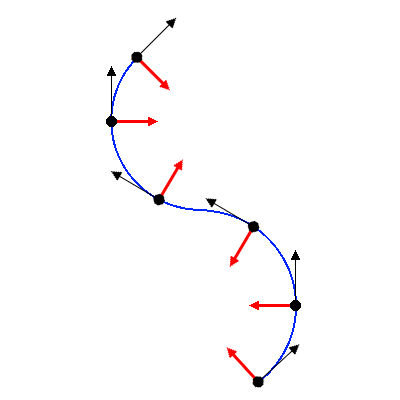
\includegraphics[width=0.5\linewidth]{figure1.png}
    \caption{Mouse movement for AD strafing \cite{MoreSteamAirstrafe}}
\end{figure}

Moving the mouse left while holding the left movement input gives some forward movement; however, in order to fully take advantage of air strafing for forward movement, the player must then follow this left movement with an equal right movement. Illustrated in figure 2, this process is commonly referred to as AD strafing because A is most commonly the left movement key and D is most commonly the right movement key. This technique of AD strafing keeps the player's acceleration always perpendicular to the velocity while fully taking advantage of the slight forward acceleration gain in both directions and although it looks confusing, is the fastest way for a player to move in source engine games \cite{AirStrafingExplained}.

In addition to emulating the acceleration and velocity, fully replicating the environment of a game engine is a difficult task. One of the main other mechanics that directly influences bunny hopping is friction. Bunny Hopping is a useful technique because friction is not calculated in the source engine on the first frame in which a player is in contact with the ground \cite{BunnyHoppingProgrammers}. Frames are fundamental units of time that represent individual snapshots of the game's state. Online multiplayer games like Counter-Strike have servers that take in input from all players in the game to calculate what is happening each tick. Counter-strike servers can calculate 64 tick per second while player's computers can render frames up to 240 times per second. The extra frames that the player's computer loads in between the server's logical ticks calculate a prediction of what each player will do and correct that prediction on receiving the next tick from the server \cite{MoreSteamAirstrafe}. Hitting the jump input on the exact frame in which a player touches the ground is very difficult and the main reason that bunny hopping is so difficult. One technique that players can use to make this easier is rebinding the jump key from the default space bar to a mouse wheel. Rolling the mouse wheel allows more inputs to be registered per second than possible by repeatedly pressing the space bar, making the technique more consistent \cite{BhopTutorialValorant}.

In Counter-Strike 2, the most current version of Counter-Strike, and its predecessor Counter-Strike Global Offensive, bunny hopping has been made significantly more difficult and less effective. The velocity cap for Counter-Strike 2 is 330 HU (Hammer Units), which is much lower than previous games. In order to combat the use of the scroll wheel to consistently hit frame perfect bunny hops, Counter-Strike 2 has also implemented a server variable called sv\_jump\_spam\_penalty\_time which prevents the use of another jump input for a brief time after an input\cite{HowToBhopCS2}. This means that using the scroll wheel to send tens or hundreds of inputs will result in less consistency than manually using a jump input. Despite these handicaps, bunny hopping is still possible in Counter-Strike 2 but requires perfect inputs. For the purpose of this paper, I will be discussing bunny hopping in Counter-Strike Source, an older Counter-Strike game that does not have measures in place to stop bunny hopping. Bunny hopping is most effective in Counter-Strike Source, and despite being released in 2004, still has a playerbase of ten thousand players per day\cite{SourceSteamCharts}.


\section{Prior work}

% bunny rabbit 1999-06-03.md
Little academic work has been done on the mechanics of bunny hopping and air strafing, but there is a significant amount of non-academic research and documentation on the evolution of these techniques. Air strafing and bunny hopping was first discovered in the video game Quake and were mechanics that the lead developer did not like. In a series of archived blogs from the developer, John Carmack he says "In the absense of powerups or level features (wind tunnels, jump pads, etc), the game characters are supposed to be badasses with big guns. Arnold Schwartzenegger and Sigourney Weaver don't get down a hallway by hopping like a bunny rabbit." \cite{CarmackPlan} As this is one of the first documented times a bunny is mentioned in reference to the technique, this blog post may be the origin of bunny hopping as a term.
He even says "Strafe jumping is an exploitable bug. Just because people have practiced hard to allow themselves to take advantage of it does not justify it's existence." The only reason it stayed as a mechanic is "When I tried fixing the code so that it just didn't work, I thought it changed the normal running movement in an unfortunate way."\cite{CarmackPlan} This blog post was written a few months before the release of Quake III but shows that this foundational mechanic of fps games was initially a bug. This is also one of many times where game developers have attempted to remove bunny hopping from their games. This developer did successfully remove bunny hopping from sequels of Quake by removing air acceleration entirely \cite{bhopHistory}.
    
As explained in the technical background section, bunny hopping and air strafing exist due to the fundamental nature of the game's engine. Despite several attempts to "fix" bunny hopping, it took several games and several years to manage properly. Half-life 2 is another game on the source engine and contains bunny hopping. The developers attempted to remove bunny hopping by adding a negative velocity whenever the player reached a high enough acceleration. What they did not account for with this solution was bunny hopping backward. This oversight introduced the mechanic of Accelerated Back Hopping, which uses the negative velocity players gain from bunny hopping to reach speeds significantly higher than possible before \cite{ABH}.

The original Counter-Strike was a player-made modification for the game Half-Life in 2000 that included the bunny hopping present in the Quake engine, with a few minor tweaks. Counter-Strike made the movement slowdown from missing the frame-perfect jump input more severe and added a movement speed cap to the player \cite{bhopHistory}. This version of bunny hopping was so popular that players created several types of maps that solely existed as obstacle courses for people to bunny hop through. Following Counter Strike was the release of Counter-Strike Source which was the first Counter-Strike game to use the source engine\cite{bhopHistory}. Counter-Strike Source maintained none of the movement penalties for bunny hopping present in Counter-Strike and, as such, was a much less competitive game \cite{ExploringEsports}. The ability for players to move so quickly made designing a map with areas designed for players to encounter one another after a few seconds of walking impossible, and players who mastered bunny hopping had significant advantages. Players who were not masters of the technique would become frustrated at players such as Phoon, a very talented player who recorded players irritation with his skill \cite{phoon}. The difference in proficiency with bunny hopping changed the game so much that competitive matches of Counter-Strike were played on the previous version. Another problem with bunny hopping at this time was scripting. Scripting is the process of running a computer script that perfectly executes a series of inputs, allowing the player to bunny hop. While detection of these scripts is very good today, in the era of Counter-Strike Source, many players who were talented at bunny hopping were assumed to be cheaters \cite{bhopHistory}. 

Counter-Strike Global Offensive or CS:GO was the first instance where the developers really cracked down on bunny hopping. As the game began to accrue more of a competitive following, professional players and developers wanted to ensure that gameplay was intuitive and understandable. The maximum velocity was lowered and the punishment for missing a bunny hop was drastically increased \cite{HowToBhopCS2}. Bunny hopping in CS:GO and Counter-Strike 2 is more of a niche technique that can be used for bursts of speed instead of allowing the player to traverse the entire map as was possible in Counter-Strike Source.

Another game, Valorant was released in 2020, 8 years after the release of CS:GO and was designed to be a tactical shooter similar to CS:GO but easier to understand and interact with. The team built their engine from the ground up and this has allowed them more control over the mechanics present \cite{devDiaries}. Even when building a game where they had the opportunity to remove the bug of bunny hopping from the game, it is such a staple of the genre that they chose to include it. Bunny hopping in Valorant is significantly easier than it is in Counter-Strike as there is no slowdown penalty for missing the frame perfect input of the jump. However, bunny hopping does not allow the player to move any faster than normal speed and is primarily used as an evasion technique or in combination with air strafing to retreat behind cover more quickly \cite{BhopTutorialValorant}. Air strafing in valorant is also unaffected by usage of the W key, making it much more intuitive than Counter-Strike air strafing.

Many Youtube videos exist that teach users how to bunny hop across various games. There are tutorials for Quake, Valorant, and all iterations of Counter-Strike. Most of these tutorials follow a similar general structure. The player will introduce the technique with a flashy clip showing its usefulness, then explain how to airstrafe and how to bunny hop \cite{QuakeBHopTutorial}. Often these guides will also give the user a helpful place to practice in game. While these tutorials are helpful, many of them lack important context and feedback necessary to understand the skill. Almost all of these tutorials mention "moving the mouse smoothly" for air strafing, which is useful but does not explain to the user the processes that are occurring and why smooth movement is important \cite{HowToBhopCS2}. The change in angle of the mouse movement is more important than the smooth movement, but in a video format is difficult to portray \cite{BhopTutorialValorant}. Many tutorials will also include statements like "as you can see its actually pretty easy," which can make the player discouraged if the technique is not as easy for them to learn \cite{QuakeBHopTutorial}. Some tutorials include visualizations of what keys are being pressed by the player, which is helpful but visualizing mouse movement is significantly more difficult and is a lacking component of most tutorials. These shortcomings of the video format are all solvable with an interactive player controlled trainer.

Aim Labs is a widely used "aim trainer" tool that allows players to practice their mouse aim by shooting virtual targets. Each scenario is typically one minute long and the goal of the activity is to hit as many targets as possible while keeping their accuracy as high as possible. This technique of isolated practice of a single aspect of a game is a large inspiration for this project and has shown to be widely used in the gaming space with 30 million players \cite{STEAMDBAimLabChart}. This technique has proved to be effective as it allows users to more quickly build muscle memory for aiming and helps train the aiming motor pathway \cite{aimTrainingWorks}. Aim Lab also gives users feedback on each task they complete and if the user is struggling with a certain aspect of their aim will suggest scenarios to train that aspect. The user feedback also gives encouraging statistics to players, congratulating them on their improvements and finding positives in their failures.


\section{Ethical Considerations}

While the goal of this project is to make an advanced technique in first person shooter games more accessible to a wide variety of people, it is important to recognize the lack of accessibility in some parts of the project. Video games are often created with a control schema that matches the developer's own ability, and many lack flexibility in gameplay options. For someone who is blind, a game that entirely relies on visual feedback is impossible to interface with. While a blind person is a clear example of someone who will struggle to use this tool, the way in which it is designed will make it difficult for people with a wide variety of limiting conditions. Despite being a tool intended to teach those with all levels of familiarity, the reliance on text prompts to relay information and data on the success of the user in the task is also a significant hurdle\cite{AccessInVidya}. Including the option for audio instruction and feedback could make the game more accessible to those with dyslexia or who are not literate. 

First-person shooters are very difficult to make accessible. Since the bunny hop trainer is a tool for teaching skills used in a first-person shooter, these accessibility concerns are inherited. As presented in the initial proposal, there is no support for controller input or any input that is not a keyboard and a mouse. Alternative input devices can be helpful tools for those who do not have the full ability to use traditional control schemes. For many people with accessibility concerns, a one-handed controller can often allow them to play a game they would not otherwise be able to. One-handed controllers are very difficult to implement for first-person shooters because they require two analog inputs simultaneously, one to control the player's movement and one to control the player's aim \cite{GameAccesibilityASurvey}. Other controllers, such as brain wave or eye-tracking controllers, are also difficult to implement for first-person shooters due to the precise nature of aiming with the mouse that it is trying to replicate. Even for those who have the ability to interface with a keyboard and mouse, the precise nature of the movements required to execute an air strafe with a mouse will further limit their ability to interface with the tool. While adding controller support would make the trainer far more accessible, Valorant and Counter-Strike are both games that do not have native support for controllers and adding this support would be a considerable undertaking. Air strafing is also requires discrete left and right inputs which are significantly harder to execute on an analog controller thumb stick. Bunny hopping is also not a necessary skill to play Counter-strike or Valorant and, in the vast majority of cases, is nothing more than a flashy technique that has no impact on the game. For these reasons I have decided not to add controller support to the first iteration of this tool.

\section{Methods}

The goal of this project is to create an app that trains new users to perform air strafes and bunny hops successfully and consistently in Counter-Strike. I created this project in the Unity game engine, an industry standard option, and used an open-source character controller by Cr4yz to model the Counter-Strike movement system in Unity\cite{fragSurf}. I started this project by creating my own character controller, but since the goal of this project was not to find magic numbers present in Counter-Strike that make its physics possible, I adapted an existing setup. Next, I split up the activity of bunny hopping into discrete skills that I could individually test and assess. The setup of these scenes were based off of other trainers in the first person shooter genre discussed earlier such as Aim Labs, where player control is limited so that they only have to focus on a very specific element of the technique.

The first scene is the bunny hop timing accuracy scene. In this scene, the player has no control of where they are looking or where they are moving, the player is constantly moving forward and the only input they have is jump. The player is instructed to jump as soon as they hit the ground for five jumps, and after the attempt is complete, they are given bunny hop timing accuracy, which is the time in milliseconds on average that they spent on the ground between jumps and their average speed. There is also an indicator in the upper left corner of the screen that shows the user where they are in their jump to give them more information about the optimal timing and help associate the timing with their position in game. 

The second scene is the look timing accuracy scene. In this scene, the player has no control of their movement or jump, only where the character is looking. The player is shown two orbs, one is 45 degrees to the left of the player, and one is 45 degrees to the right of the player. The player is instructed to start by looking at the left orb and move their crosshair on to the right orb and back to the left orb with the same timing as the first scene. The same indicator as the first scene is present here. The user receives feedback on their look timing accuracy, which is the difference in milliseconds on average from the optimal timing for each attempt to switch targets. They also receive feedback on their aim smoothness, which is a metric for how gradually they moved their view between targets. If the player were to move 85 degrees in 0.05 seconds and then 5 degrees over the next 0.6 seconds, their score would be very bad, but if they moved 1.4 degrees each 0.01 seconds they would receive a perfect score.

The third scene is the strafing timing accuracy scene. Similar to the second scene, the player has no control of their movement or jump, only where the character is looking. The player is shown two orbs, one is 45 degrees to the left of the player, and one is 45 degrees to the right of the player. In this scene, the player is instructed to change which orb they are looking at with the optimal timing, but additionally, whenever the player is looking right they should hold the D key and whenever the player is looking left they should hold the A key. The user receives feedback on look timing accuracy but also strafing timing accuracy. Strafing timing accuracy is the difference in milliseconds on average from the time  which the player changed look directions and the time in which the player started pressing the corresponding key.

Now that I have laid out the individual scenes, I will discuss decisions that were made throughout the project and the process of creating the optimal scenes and metrics for each scene. While my original goal was still to isolate individual elements of the skill into separate scenes, my first iteration of the scenes was confusing to new players. My first scenes had the player character fully performing the correct actions of bunny hopping regardless of input, which made it difficult to focus on the individual elements. For example, in the look accuracy scene, the player character would automatically jump, move forward and hold right, while the player was supposed to move their mouse to the right. After doing initial user testing without results to see what new players found intuitive, I changed the scenes to be more visually simple, and help the user focus more on the individual skill. Throughout my project, I had several rounds of user testing with new users before recording data to make sure that my tool was easy to understand. While many of these resulted in helpful feedback, such as simplifying the visual elements of the scene, some recommendations were not as helpful. One suggestion that was offered by several users was the addition of a restart button, as they would become discouraged upon missing an input. While I understand the desire for a restart button, adding one would make the process of determining user improvement for the purpose of evaluation fraudulent, and would make the statistics shown to the player after attempts less accurate. Another suggestion, which would require significant expansion of the project, was adding leaderboards to see who had the highest scores in individual scenes. These two suggestions go hand in hand, as a restart button would be very helpful in achieving high scores, but as my tool is focused more on improvement than fun, it is currently outside of the scope of this project.

The most difficult part of the development of this tool was accurate recording of the relevant statistics as well as determining which metrics were most useful as statistics for both the player and evaluation. Some statistics, such as bunny hop timing accuracy were clear, as bunny hopping on the first frame is necessary for the skill, so minimizing the time on the ground makes sense as a metric. Strafing timing accuracy seemed simple, as a perfect strafe is executed at the same time as a jump, but in reality, a perfect strafe should be performed at the same time as a change in look direction, which may not be at the same time as a jump. Originally, I calculated the offset of Strafe direction from the jump time, but this led to situations where people would have good scores for strafe timing but would be moving slower. Now, in order to calculate the most relevant strafe, I record the timestamp each time the strafe key was pressed and calculated the closest strafe to the change in look direction. To calculate the offset I found the difference between the two times. Change in look direction is another element that was more difficult to determine than expected, as humans are not good at moving the mouse in a perfectly straight line, often times when moving to the right they might move a degree or two to the left, so I checked for a three degree change in the opposite direction every 0.01 seconds as an indication of change in direction. 

\begin{figure}
    \centering
    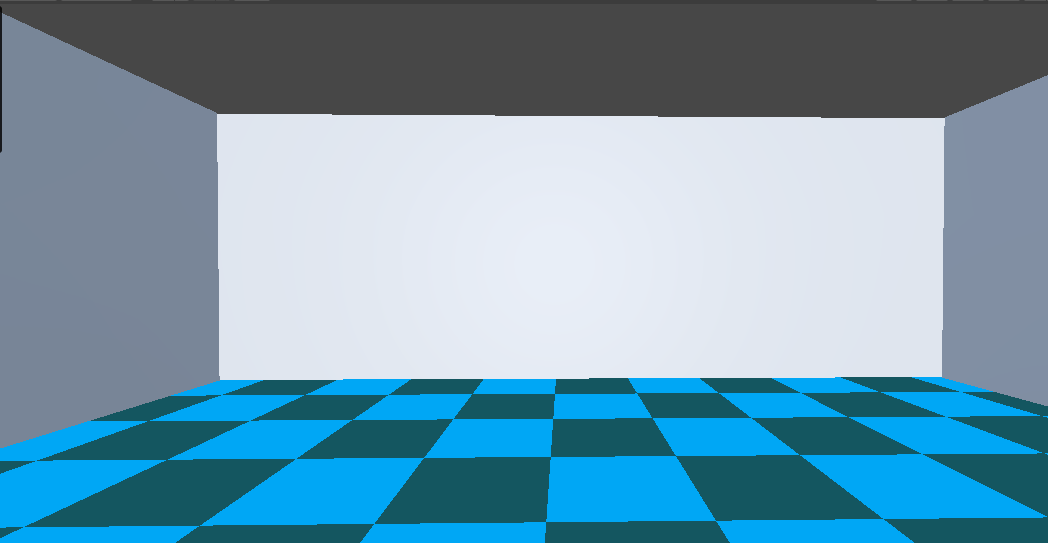
\includegraphics[width=1\linewidth]{gameEnvironment.png}
    \caption{Game Environment}
\end{figure}
\begin{figure}
    \centering
    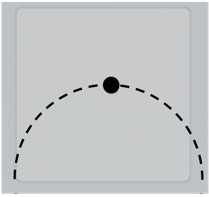
\includegraphics[width=0.5\linewidth]{JumpIndidcator.png}
    \caption{Jump Indicator}
\end{figure}

I also spent a significant amount of time developing a user interface that made sense for conveying information to the player. For the game environment I decided on a blue and black checkerboard pattern with plain white walls to avoid distractions. The checkerboard, shown in Figure 3 is also a useful tool for players to understand how far they are moving with each jump. Another element of the user interface that took refinement was the jump indicator. I wanted to inform the player of the optimal timing for bunny hopping that accounts for the player missing a jump. An original approach was to have an element near the center of the screen that changes color when it is time to jump, but this does not help players predict when a jump is coming, and felt confusing. My next attempt used a series of moving lines in a box that would spawn when the player jumped, and crossed over the middle of the box when the player touched the ground. This approach had too many moving parts and was confusing. My final indicator, shown in figure 4, spawns a dot in the bottom left corner that follows an arc similar to the player's, landing on the right when the player should start their next jump. 

\begin{figure}
    \centering
    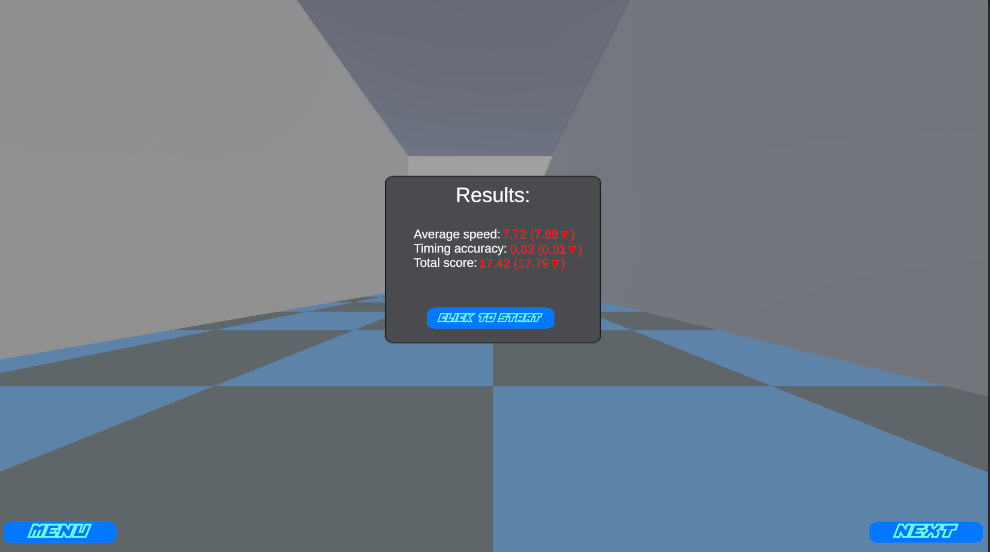
\includegraphics[width=1\linewidth]{resultsScreen.png}
    \caption{Negative results from scene 1}
\end{figure}
\begin{figure}
    \centering
    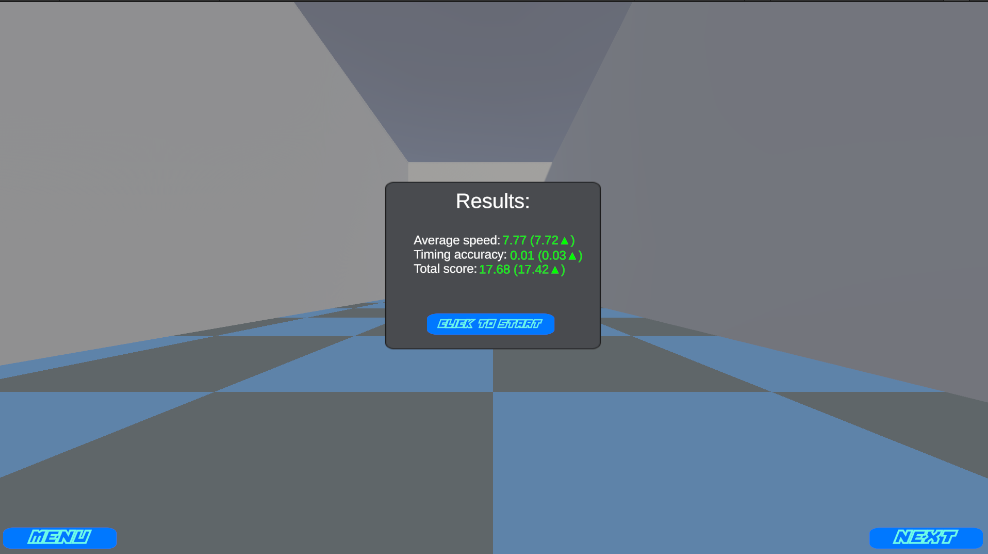
\includegraphics[width=1\linewidth]{resultsGood.png}
    \caption{Positive results from scene 1}
\end{figure}

Another important element of the tool is the results screen, where the user learns how they did in their attempt. The process of choosing the relevant metrics for each scene went hand in hand with developing the stats screen for each scene. I added a grey overlay to differentiate the stats from the game environment, and added a box in the middle. Originally I had a "good" score listed to give users an idea of what they should aim for, but after learning about the potential impact a negative mindset, such as one created by unrealistic expectations, could have, I removed them \cite{learningOptimal}. I landed on a system that compares the user's current attempt to their most recent attempt of that scene and provides an up arrow with green text as shown in Figure 6 if the user had improvement, and a down arrow with red text as shown in figure 5 if the user did not improve. I also wanted to present the user with real time feedback wherever possible, so in the strafing and looking scenes, the orb will change color based on how accurate the look offset was. Green represents a look offset of .1 or lower, yellow is .1 to .2 and red is .21 or higher. An accurate look attempt can be seen in figure 7. Also present in figure 7 is a crosshair that helps the user determine where they are looking, and an arrow that tells the user which direction they should be looking. 
\begin{figure}
    \centering
    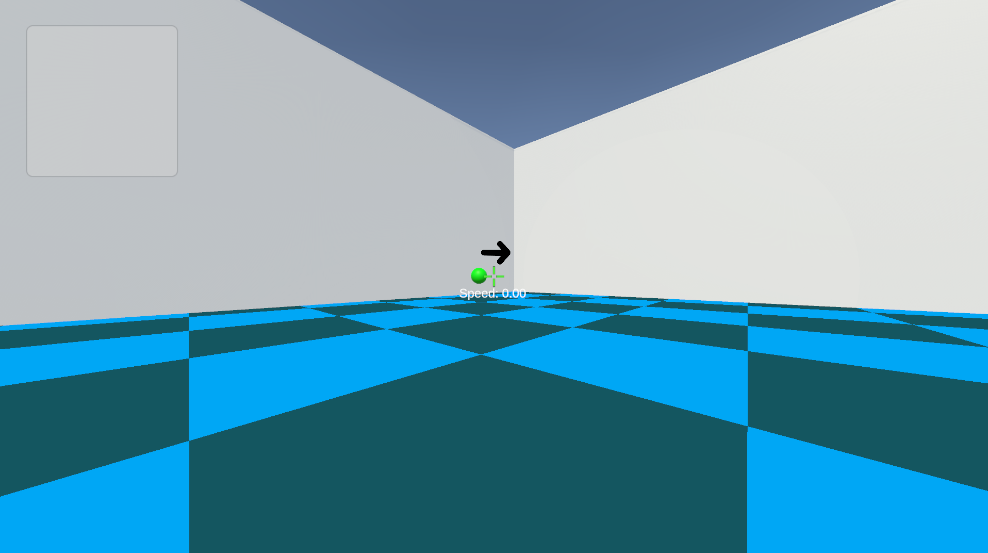
\includegraphics[width=1\linewidth]{greenOrb.png}
    \caption{An Accurate Look Attempt}
\end{figure}

\section{Evaluation metrics}

The goal of this project is to create a tool that allows users to learn how to bunny hop or improve their consistency with that skill. One of the core elements of my tool is the ability for users to see relevant statistics about each attempt they complete and their progress between attempts. I created a Json file for each scene for each user to track each statistic for each scene. My recorded metrics were discussed in the methods section, but the most important metrics for evaluation overall are speed and time to complete. While a visually pleasing user interface is a necessary part of a product, the goal of this project is to create a tool that improves player skill, so this will not be an area that is evaluated.

For my evaluations, in order to establish a baseline metric for player skill, each user was instructed on how to bunny hop and provided a video to show them how the skill was performed. This is supposed to simulate the currently available methods of learning to bunny hop. The user was then asked to perform three attempts of a "race" scene that assesses the player's average speed, bunny hop timing accuracy, strafing accuracy, look accuracy, and time to move from a start line to a finish line. In this scene, average speed is the most useful metric, as the goal of bunny hopping is to generate and conserve as much speed as possible, and is the most comparable across users. After the race scene, the user was guided through the four scenes described above to give the player practice on individual elements of bunny hopping. After practicing each individual mechanic, the user completed three more attempts of the race scene to record their progress. While the ideal usage of this trainer involves practicing for twenty to thirty minutes per day, getting a full testing group with this commitment level was outside of the scope for this project, and an abridged version where each user performed five to ten attempts of each training exercise was used. It has been shown that learning a motor skill is most effective when the user does focused practice consistently, strengthening the neural pathways used in the activity \cite{learningOptimal}. I also asked each user what first person shooter they most often play, and their level of proficiency with bunny hopping, as the goal of this tool is to teach bunny hopping specifically in Counter Strike and games that share its movement system. For my user selection criteria I selected users who are familiar with the control scheme of first person shooters, but unfamiliar with how to perform the technique of bunny hopping. 

This project will be considered successful if there is improvement of ten percent in overall forward speed and time to complete on average between the first three race attempts and the second three race attempts and a average forward speed higher than the forward run speed of 7.15 units/second. If average forward speed is above the normal run speed, bunny hopping is a more efficient method of movement than running and would be advantageous to use in game. Time to complete is also a useful metric as it shows how much faster the user completed the entire race. While bunny hop timing accuracy is a  useful metric for a longer test over several days, the consistency required to hit perfect bunny hops ten times in a row or higher is very difficult in such a short learning period. Comparing forward speed to run speed and using time to complete as a metric gives a better understanding of whether learning the technique makes it more efficient than running in the game, which is the ultimate goal of bunny hopping. 

While it is useful to look at each individual metric recorded in their individual scenes, the skill of bunny hopping is ultimately a combination of all components and looking at an average of bunny hop accuracy, strafe timing accuracy, and look timing accuracy across all jumps in the race scene does not give an accurate enough representation of what exactly went wrong or right. It is useful however, to look at individual metrics in their specific scenes to see if there was progress in each scene, and how that progress took place.

\section{Results and Discussion}

\begin{figure}
    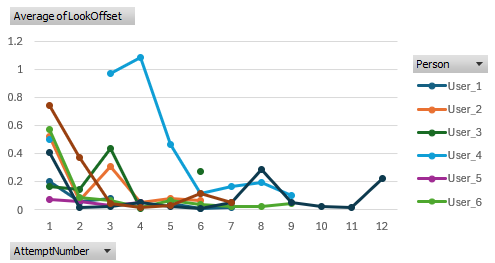
\includegraphics[width=1\linewidth]{LookOffsetGraph.png}
    \caption{Graph for Change in LookOffset for Scene 1}
\end{figure}
I tested eight different people for this project as the available group of users who fit my selection criteria was relatively small. On average, Users who tested my project increased their speed over the course of the tests by 23\% as shown in figure 9, which I found statistically significant usin a t-test with a P value of 0.000332. Improvement in each scene was also found, as shown in figure 8, which represents improvement in the look attempt scene.

\begin{figure}
    \centering
    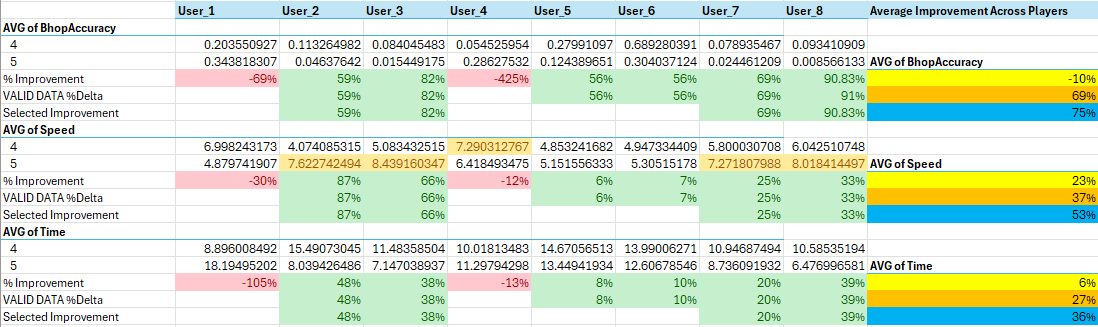
\includegraphics[width=1\linewidth]{RaceData.png}
    \caption{Race Scene Before (4) and After Training (5)}
\end{figure}

User\_1 and User\_4 were invalid datapoints. User\_1 was not confident in their performance, and did not attempt to bunny hop in the first race attempt, and panicked and paused in their second race attempts. User\_4 consistently walked backwards to the start line after jumping incorrectly in the second race scene, which interfered with their data. Due to the nature of the project, I could not re-run the test with these users as the goal of this project is to test how users learn, and testing after a user has already learned will not be useful. After removing these invalid data points, the average improvement significantly increases. Average speed improved by 37\%, and average time improved by 27\%. After performing a t-test on both of these values, both are statistically significant and show considerable improvement after using my tool.

I tested users most familiar with several different games, User\_1 and User\_5 are most familiar with Overwatch 2, User\_4 is most familiar with Apex Legends, and User\_6 is most familiar with Fortnite.  User\_2, User\_3, User\_7, and User\_8 are all most familiar with Counter-Strike, these users are my main target group for this evaluation as they are the target group for this tool. When selecting for only the main target group, average speed improved by 53\%, and average time improved by 36\%, both of which are statistically significant according to a t-test. 

As discussed in the technical background section, bunny hopping in Counter-Strike is only possible due to several very specific properties of the Source engine physics system \cite{BunnyHoppingProgrammers}. Games like Overwatch and fortnite do not slow the user's speed in the air while holding the W key, while pressing the W key for even a few frames in this environment removes the acceleration gain. In Apex Legends, there is even a mechanic called "tap-strafing," in which the player repeatedly taps the W key to gain significant amounts of speed and movement while air strafing \cite{TapStrafing}. With these significant changes in gameplay environment that users 1, 4, 5 and 6 had to learn, it makes sense that they would have a more difficult time learning a new skill. This was also a problem I ran into when attempting to test a set of users who were familiar with bunny hopping in other game environments. The first user I tested, who mainly plays the game "UltraKill", a game where in order to conserve speed most effectively, the user holds the strafe key that is opposite to the direction they are moving. This behavior is exactly opposite the optimal behavior for bunny hopping in Counter-Strike and caused the user to move backwards instead of forwards. For all users who have hundreds of hours of muscle memory from other games, learning a new way of moving is difficult.

It is certainly possible and likely that repeated practice of the activity was helpful and therefore improved the user's performance. This level of influence of practicing the activity is difficult to control for as each user entered with a different starting point and learns at different speed, but with the significant improvement shown, the trainer is significant. To greater prove the trainer's significance it is helpful to look at how Users improved in individual scenes. The missing attempts are attempts that were interrupted in the middle, due to a pause or a change in user sensitivity.  Interestingly, in Figure 8, several users had an attempt where their performance significantly worsened before it got better. From observation, this occurred once the user felt comfortable with the exercise and got into a rhythm. After getting into a rhythm, the user would miss the correct angle for a look attempt, but continue the exercise, which caused them to have one very high lookOffset value. In turn this value would cause a high average value for this attempt. This occurrence can be most clearly observed on attempt 3, attempt 6 and attempt 8. It would be interesting to see how changes in learning could be observed differently in a longer test.

The goal of this project was to teach Counter-Strike players how to bunny hop in a way that would be helpful in that game. The Counter-Strike players on average ended with an average forward speed of 7.32, significantly higher than the base run speed of 7.15, which indicates that this technique would be useful in game. The study conducted also showed that players improved on individual mechanics in individual scenes, and even that non-Counter-Strike players were still able to improve significantly in speed and time to complete with the help of this tool. With the data collected, I can confidently say that the bhop trainer was successful in teaching people how to bhop at a level that would be useful in Counter-Strike.
    

\printbibliography

\appendix
\section{Replication Instructions}
To run the full bhop trainer, you can run the "Comps Project Bhop Trainer.exe" file under the "builds" folder in the github project. This project is working as of Microsoft Windows 11 Home version 10.0.22631, which is the version it was created in. Saved Json data for viewing attempts by default will save to "C:\textbackslash{}Users\textbackslash{}User\textbackslash{}AppData\textbackslash{}LocalLow\textbackslash{}DefaultCompany\textbackslash{} Comps Project Bhop Trainer." Sensitivity in settings is set to Counter-Strike 2 sensitivity and the scroll wheel or space bar can be used to jump. If you would like to edit the project, you must download Unity Hub (currently available on the Unity website) and install version 2022.3.44f1. 

\section{Code Architecture Overview}
The trainer is made up of a series of c\# script files and Unity project gameObjects. Each scene has its own GameManager script and scene in Unity. There is also a playerManager that manages the player and its relevant characteristics, a scoreManager that manages loading and saving scores from JSON, a UI manager that manages which UI elements are on screen, and an orbController for the look and strafing scenes. The player character also has a speed tracker script and Z speed tracker script to keep track of average player speed and a mouseAngleTracker script to keep track of the player's current mouse angle and the change in mouse angle over the attempt. The player character also has the surfCharacter script, which manages the player's movement, and a cameraHolder child that has a playerAiming script that allows the player to control the camera with the mouse. 

The canvas holds all of the UI elements for the game and organizes them into four subPanels, HudElements, StartElements, AfterStats, and SettingsPanel. The UI manager controls which subPanel is active during runtime. HudElements contains elements present during gameplay such as the crosshair, the jumpIndicator, and the arrow telling the player which way to strafe. StartElements contains the description of the scene and the button to start the scene. AfterStats contains a box and the text that tells the player how they performed relative to the previous attempt. The stats for AfterStats are populated by a StatScreen script unique to each scene, AimingStatScreen or StrafeStatScreen for example. SettingsPanel is the toggleable settings menu that can be accessed to change the system settings at any time and is a singleton object that saves to a JSON file.

Each scene is modeled using unity gameObjects, and various scripts in the SurfCharacter and PlayerManager are called by the GameManager script for the given scene to enable or disable movement, aiming, or other control of the player. There are also button GameObjects in each scene that change the scene by loading another scene through the onClick field exposed in Unity. 

\begin{figure}
    \centering
    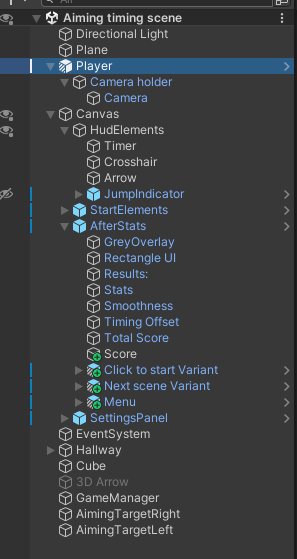
\includegraphics[width=1\linewidth]{UnityEditor.png}
    \caption{Unity Editor Hierarchy}
\end{figure}
The layout of each scene and the parenting of each gameObject and script can be easily seen in the Unity editor in Figure 6. For expanding this project into more scenes, this layout could be copied and the AimingTimingSceneManager could be adapted to the new scene's functionality. This project was intentionally designed to have components that can exist without other scripts to make expansion and adaptation easy, as I had to design five separate scenes. Using the different SceneManagers that already exist, creating a new scene should be relatively straightforward.

\end{document}
